% Chapter Template

\chapter{Dashboard} % Main chapter title

\label{DissenyDashboard} % Change X to a consecutive number; for referencing this chapter elsewhere, use \ref{ChapterX}

Com a complement addicional al desenvolupament del projecte, es defineix la implementació d'un \textit{dashboard} en mitjà d'aplicació web que ens permeti interactuar amb el nostre sistema per tal de, mitjançant una usabilitat molt bàsica i senzilla, poder executar reconfiguracions i visualitzar les diferents adaptacions que s'han realitzat. Buscarem, per tant, un disseny senzill que no requereixi una gran dedicació del projecte (ja que entenem que no és una prioritat), però si que ens permeti la interacció necessària per poder satisfer aquesta necessitat.

\section{Anàlisi de requisits}

Per satisfer aquest objectiu, volem que el nostre \textit{dashboard} satisfaci les següents necessitats:

\begin{itemize}
\item \textbf{Visualitar propostes d'adaptacions.} A través dels models definits al Model Repository, permetre mostrar les dades principals de cada \textbf{Feature Configuration} emmagatzemada al nostre sistema.
\item \textbf{Executar una adaptació.} A partir del llistat de \textit{Feature Configurations} anterior, el \textit{dashboard} ha de permetre a l'usuari seleccionar una proposta d'adaptació i demanar la seva execució al sistema corresponent. Aquesta serà la interacció principal, que ens permetrà executar els casos de validació de la reconfiguració del nostre sistema de monitoratge. 
\item \textbf{Visualitzar adaptacions executades.} Com en la 1a vista, permetre mostrar les dades principals de cada \textbf{Feature Configuration} amb \textit{status == Enacted}, i per tant executada.
\end{itemize}

Des d'un punt de vista funcional, els requisits són relativament senzills, ja que traduït a necessitats de disseny i implementació únicament caldrà definir dues vistes i una interacció amb l'usuari, que es reprodueixi en una interacció amb l'Adapter. Aquesta interacció, com en la resta de casos, es realitza a través de l'eina IF.

\section{Disseny de la interfície}

Partint dels requisits anteriors, necessitem definir dues vistes a la interfície: la vista de \textbf{adaptacions suggerides} i \textbf{adaptacions executades}.\\

\begin{figure}
\centering
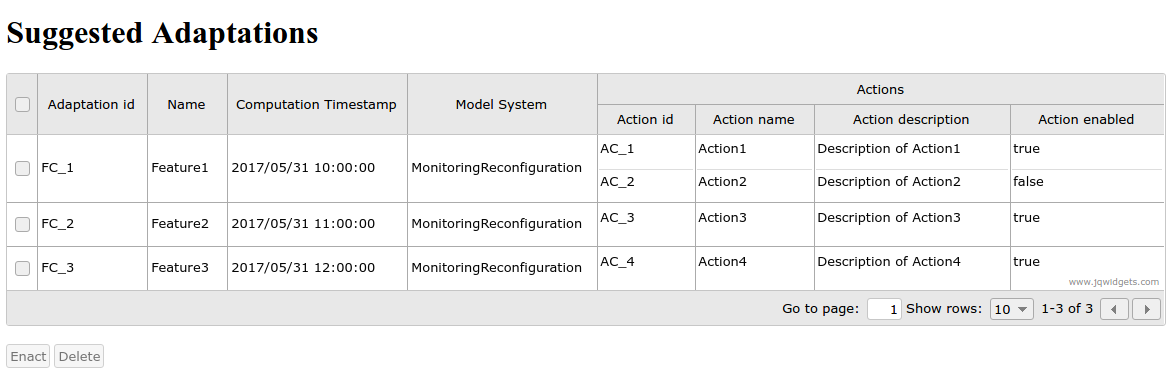
\includegraphics[width=14cm]{Figures/Figure32}
\decoRule
\caption{Disseny de la vista d'adaptacions suggerides del \textit{dashboard}}
\label{fig:Figura32}
\end{figure}  

La vista d'adaptacions suggerides consisteix en una taula on cada fila representa una d'aquestes entitats (i, per tant, una \textit{Feature Configuration} del sistema). Per cada instància, mostrarem les següents dades:

\begin{itemize}
\item \textbf{Adaptation id}. Identificador de la \textit{Feature Configuration} que representa
\item \textbf{Name}. Nom únic associat a aquella \textit{Feature Configuration}, usualment associat semànticament a les seves característiques 
\item \textbf{Computation timestamp}. \textit{Timestamp} de la creació de la \textit{Feature Configuration}. Ens serveix per ubicar temporalment les diferents configuracions creades
\item \textbf{Actions}. Cada \textit{Feature Configuration} defineix una sèrie de \textit{features}, o accions, que s'activen o desactiven en funció de les seves característiques. Per cada acció a aplicar, mostrarem:
\begin{itemize}
\item \textbf{Action id}. Identificador de l'acció a realitzar
\item \textbf{Action name}. Nom únic per aquella \textit{Feature Configuration} que rep l'acció o \textit{feature} a modificar
\item \textbf{Action description}. Descripció textual que defineix la modificació i canvis implicats per aquella acció
\item \textbf{Action enabled}. Indica si l'acció indica l'activació d'una \textit{feature} (true) o la seva desactivació (false).
\end{itemize}
\end{itemize}

Addicionalment, en aquesta vista cal contemplar el 2n requisit funcional d'\textbf{execució d'una adaptació}. Mitjançant la selecció d'una de les adaptacions suggerides al nostre sistema (és a dir, la selecció d'una fila a la taula), afegim un botó a la part inferior esquerra amb l'etiqueta \textit{"Enact"}. Aquesta interacció activa la comunicació amb l'Adapter, i inicia l'algorisme d'adaptació de models (en aquest cas, no de forma completament automàtica, sinó donada una \textit{Feature Configuration} específica). Com a resultat, una nova adaptació s'executa al nostre sistema; s'actualitzaran les dades al Model Repository, que podem consultar a través del \textit{dashboard}, i es modificarà l'acció real dels components adaptats (monitors pel nostre cas), d'acord amb les modificacions anteriors.\\

En aquesta segona vista d'adaptacions executades, mostrarem de forma paral·lela al disseny anterior una taula on cada fila representa una \textit{Feature Configuration}, però aquest cop que ja ha estat executada al nostre sistema. Mostrarem algunes de les dades bàsiques d'aquella \textit{Feature Configuration}, com en el cas anterior, però afegirem les següents dades:

\begin{itemize}
\item \textbf{Enactment request time}. \textit{Timestamp} que conté la data i hora en què s'ha realitzat la petició d'execució de l'adaptació
\item \textbf{Enactment completion time}. Mostra el temps total de l'execució d'aquesta reconfiguració, amb una precisió de mil·lisegons. 
\item \textbf{Result}. Indica si l'adaptació s'ha realitzat satisfactòriament (SUCCESS) o bé si s'ha produït algun error (FAILURE).
\end{itemize}

\begin{figure}
\centering
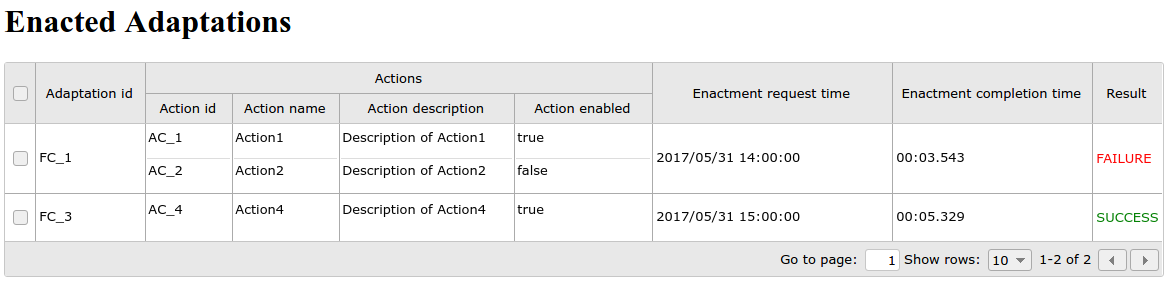
\includegraphics[width=14cm]{Figures/Figure33}
\decoRule
\caption{Disseny de la vista d'adaptacions executades del \textit{dashboard}}
\label{fig:Figura33}
\end{figure} 

Complementàriament s'ha afegit l'opció d'eliminar una entitat (adaptació suggerida o executada) en cada vista, amb objectius orientats al desenvolupament i al testeig de l'aplicació.\\

Amb aquestes dades i amb la interacció definida, tenim un component bàsic usable que ens permetrà executar les reconfiguracions del sistema de monitoratge.

\section{Implementació}

La implementació del \textit{dashboard} consisteix en l'extensió d'un projecte pare definit com el \textit{front-end} del projecte SUPERSEDE. Aquest projecte consisteix en una aplicació web desenvolupada amb \textit{Spring Framework}, que permet el desenvolupament d'aplicacions web i la gestió i \textit{mapping} de persistència. Per desenvolupar el \textit{dashboard} per la reconfiguració de models, implementarem un projecte que actuarà de submòdul dins aquest \textit{front-end}.\\

Seguint l'arquitectura proposada pel desenvolupament d'aplicacions web amb Spring, a la figura ~\ref{fig:Figura34} podem veure el disseny del domini disseny i implementat al \textit{dashboard}. Primerament, cal definir les classes de domini que representen les diferents entitats presents al \textit{dashboard}. Distingirem entre \textit{Adaptation} com a entitat que representa una \textit{Feature Configuration} suggerida, i \textit{Enactment}, que representa una \textit{Feature Configuration} executada. Addicionalment, i per millorar el disseny, definirem l'entitat \textit{Action}, ja introduïda anteriorment, del qual una \textit{Adaptation} en pot tenir vàries instàncies. Per cadascuna d'aquestes classes de domini (amb els atributs definits anteriorment), cal implementar una extensió de \textit{JpaRepository}, que actuen com a controladors de la capa de domini \cite{jpa}. Es tracta de classes que ofereix el framework Spring, i que defineix les operacions bàsiques per les classes de domini (operacions CRUD bàsicament).\\

\begin{figure}
\centering
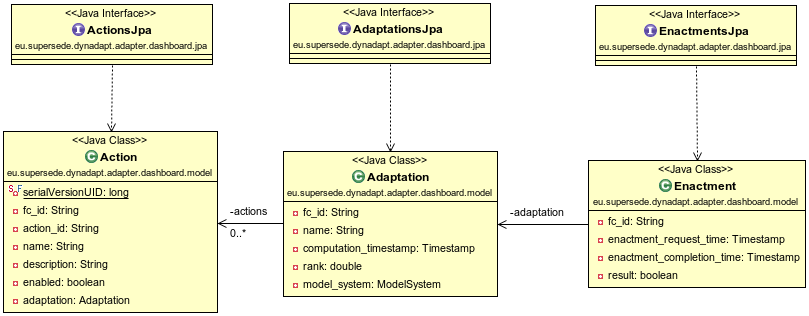
\includegraphics[width=14cm]{Figures/Figure34}
\decoRule
\caption{Disseny del domini del \textit{dashboard}}
\label{fig:Figura34}
\end{figure} 

Addicionalment, per implementar les vistes i l'aplicació web necessitem definir un controlador RESTful que s'utilitzarà per invocar els diferents mètodes del \textit{dashboard} des de la pròpia aplicació. A la figura ~\ref{fig:Figura35} podem veure els 3 controladors i les operacions implementades. Generalment aquestes estan orientades a test i validació, i únicament 5 seran utilitzades dins el context de l'aplicació: \textit{getAdaptations(),} \textit{deleteAdaptation()}, \textit{enactAdaptation()}, \textit{getEnactments()} i \textit{deleteEnactment()}. Cadascun d'aquests mètodes utilitza els repositoris implementats amb la lògica addicional necessària per satisfer la seva funcionalitat, com és el cas de l'operació \textit{enactAdaptation}, que es comunica a través de IF amb l'Adapter.

\begin{figure}
\centering
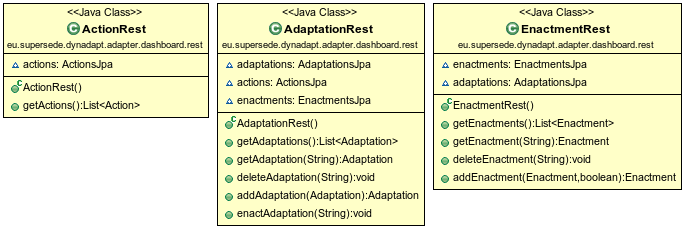
\includegraphics[width=14cm]{Figures/Figure35}
\decoRule
\caption{Disseny dels controladors REST del \textit{dashboard}}
\label{fig:Figura35}
\end{figure} 